\documentclass{article}
\usepackage[preprint]{neurips_2024}
\usepackage{microtype}
\usepackage{subcaption}
\usepackage{multirow}
\usepackage{array}

\graphicspath{{../figures/}}

% ── Metadata ──────────────────────────────────────────────────────────────────
\title{Survival Analysis of Achilles Tendon Rupture Risk in NBA Athletes:\\
A Competing-Risks Deep Learning Approach with Workload Features}

\author{%
  Solia Valentine \\
  Independent Researcher \\
  \texttt{soliavalentine@gmail.com}
}

% ══════════════════════════════════════════════════════════════════════════════
\begin{document}
\maketitle

% ── Abstract ──────────────────────────────────────────────────────────────────
\begin{abstract}
Achilles tendon rupture is among the most career-altering injuries in
professional basketball, with roughly one in five affected players failing to
return to their prior performance level.  Existing machine learning approaches
to NBA injury prediction rely on binary classification over season-level
aggregates, ignoring right-censoring, competing risks, and the temporal
structure of workload accumulation.  We present the first survival analysis
model for NBA Achilles rupture risk, applying the DeepHit competing-risks
framework to 132 player-seasons (33 ruptures, 99 position-matched controls,
2010--2026).  Game-log features are engineered via exponentially weighted
moving-average acute:chronic workload ratios (EWMA-ACWR) at three window
scales.  The model achieves a Harrell C-index of \textbf{0.81} on a temporally
held-out case-control test set, compared to 0.46 for a demographics-only
baseline.  SHAP feature attribution reveals that load and recovery features
occupy 4 of the top 5 predictive positions; the first demographic predictor
ranks 5th at $6\times$ lower importance than the top feature, consistent with
\citet{gabbett2016}.  We additionally introduce the design of an NLP weak-supervision
pipeline using Snorkel \citep{ratner2017snorkel} and BioBERT for prodromal
injury window identification, to be validated in future work.  Code is publicly
available.\footnote{\url{https://github.com/soliavalentine/nba-achilles-survival}}
\end{abstract}

% ── 1. Introduction ───────────────────────────────────────────────────────────
\section{Introduction}
\label{sec:intro}

Achilles tendon rupture (ATR) is a low-incidence, high-consequence injury in
professional basketball.  The 2019 NBA Finals produced two consecutive ruptures
---Kevin Durant and Klay Thompson of the Golden State Warriors---illustrating
both the unpredictability of the injury and its potential to alter the
competitive landscape of an entire season.  Epidemiological studies estimate
that fewer than 80\% of affected NBA players return to the same performance
tier, with career earnings losses exceeding \$10 million per event in severe
cases \citep{torresronda2022}.

From a machine learning standpoint, ATR prediction presents three difficulties
not addressed by standard binary classification.  First, \textbf{right
censoring}: most players observed across a given season do not rupture, but
they remain at risk for future seasons.  A model trained on season-level
outcome labels discards this temporal information.  Second, \textbf{competing
risks}: a player may exit the cohort due to ATR, retirement, or another
career-ending injury; ignoring competing events inflates estimated ATR
probabilities \citep{lee2018deephit}.  Third, \textbf{temporal workload
structure}: the sports-science literature establishes that injury risk is
driven not by a single point-in-time load value, but by the \emph{ratio} of
recent to habitual load over multiple time horizons \citep{gabbett2016}.

Existing NBA injury prediction work \citep{cohan2021,lu2022} applies binary
classification over season-aggregated statistics, losing the ability to
identify the specific weeks or games of elevated risk that would enable
actionable load management interventions.  Achilles-specific ML work
\citep{kapinski2024} uses MRI-derived features available only at clinical
evaluation, not during an ongoing season.

We address these gaps with the following contributions:
\begin{enumerate}\itemsep0pt
  \item \textbf{First survival analysis model for NBA ATR risk}, using the
        DeepHit competing-risks framework \citep{lee2018deephit} with
        properly censored longitudinal follow-up.
  \item \textbf{EWMA-ACWR feature engineering} adapted to NBA game-log data at
        three window scales (3:21, 7:28, and 14:56 days), preserving temporal
        workload structure that single-observation metrics discard.
  \item \textbf{Temporal train/val/test split} preserving causal ordering (no
        post-injury data visible during training), yielding an honest held-out
        case-control C-index of 0.81 on the 2022+ cohort.
  \item \textbf{SHAP-based feature attribution} quantifying the relative
        contribution of workload versus demographic features, confirming the
        ACWR hypothesis in an NBA-specific competing-risks framework.
\end{enumerate}

% ── 2. Related Work ───────────────────────────────────────────────────────────
\section{Related Work}
\label{sec:related}

\paragraph{NBA injury prediction.}
\citet{cohan2021} apply convolutional and recurrent networks to general NBA
injury prediction, using binary labels over full season windows.
\citet{lu2022} examine lower-extremity injuries specifically, using tabular
features drawn from play-by-play and biometric data.  Neither work models
right-censored time-to-event outcomes or accounts for competing risks, and
neither focuses on the Achilles tendon as a specific target.

\paragraph{Achilles tendon ML.}
\citet{kapinski2024} predict rupture risk from MRI morphological features and
collagen genetic variants \citep{september2012}, achieving good discrimination
in a clinical cohort.  MRI features are unavailable in a real-time NBA training
context, motivating game-log-based approaches.  \citet{li2025} propose a
multimodal framework for soft-tissue injury prediction across multiple sports,
though not NBA-specific and not survival-based.

\paragraph{Workload and injury: ACWR.}
\citet{gabbett2016} established the acute:chronic workload ratio as the primary
modifiable predictor of soft-tissue injury across elite sports, reporting that
athletes with ACWR $>$ 1.5 face substantially elevated injury probability.  Our
EWMA formulation follows the exponential-decay generalization recommended by
subsequent meta-analyses, which reduces boundary artefacts present in simple
rolling-window ACWR \citep{torresronda2022}.

\paragraph{Survival analysis and competing risks.}
\citet{lee2018deephit} introduce DeepHit, a deep learning survival model that
jointly learns the joint distribution over event times and event types without
imposing a proportional-hazards assumption.  The architecture outputs a
cause-specific probability mass function over discretised time bins, enabling
direct computation of cause-specific cumulative incidence functions (CIFs).
We adopt DeepHit as our base architecture given its flexibility for small
datasets and its built-in competing-risks treatment.

% ── 3. Methods ────────────────────────────────────────────────────────────────
\section{Methods}
\label{sec:methods}

\subsection{Data Collection and Cohort Construction}
\label{sec:data}

\paragraph{Ground truth.}
We scrape ProSportsTransactions.com for all NBA injured-list (IL) placements
mentioning Achilles-related keywords (2010--2026), yielding 291 records.
A three-class severity classifier is applied to free-text IL notes using
keyword matching in priority order: \textit{rupture} $\leftarrow$
\{``rupture'', ``torn'', ``surgery'', ``out for the season''\};
\textit{tendinopathy} $\leftarrow$ \{``tendinitis'', ``tendinopathy'',
``soreness'', ``day-to-day''\}; else \textit{unspecified}.  After
deduplication to the first IL placement per player (removing follow-up
``recovering from surgery'' entries), we obtain \textbf{33 confirmed Achilles
rupture events} spanning 2010--2026.

\paragraph{Control matching.}
For each rupture event, we select 3 position-matched controls from the same NBA
season: players of the same broad position (Guard / Forward / Center) who
appeared in at least one game that season and did not rupture.  Controls are
randomly sampled from season rosters retrieved via the NBA Stats API.
This yields \textbf{99 matched controls} and a cohort of 132 player-seasons.

\paragraph{Temporal split.}
To prevent data leakage, we partition by observation year: training set
(pre-2020: 79 rows, 22 events), validation set (2020--21: 17 rows, 2 events),
and test set (2022+: 36 rows, 9 events).  The test set is held out until final
evaluation and is never used for model selection.

\subsection{Feature Engineering}
\label{sec:features}

\paragraph{EWMA-ACWR.}
For each player, we retrieve game-by-game logs (minutes played, FGA, FTA, PTS)
via the NBA Stats API for the 3 seasons preceding the observation date.  We
insert zero-load entries on calendar days without games to enable
time-continuous EWMA decay, a refinement over simple rolling-window ACWR that
eliminates boundary artefacts at window edges.  The EWMA-ACWR at window scale
$(a, c)$ is:
\begin{equation}
  \text{ACWR}_{a,c}(t) = \frac{\text{EWMA}_a(t)}{\text{EWMA}_c(t)},
  \quad
  \text{EWMA}_{\tau}(t) = \frac{\sum_{s \leq t} w_{\tau}(t-s)\,L(s)}
                               {\sum_{s \leq t} w_{\tau}(t-s)},
  \quad
  w_{\tau}(\delta) = \left(\frac{\tau-1}{\tau+1}\right)^{\!\delta}
  \label{eq:ewma}
\end{equation}
where $L(s)$ is the load (minutes played) on day $s$ and the EWMA span
parameter is $\tau = 2d - 1$ for window width $d$.  We compute three scales:
$(a, c) \in \{(3,21),\,(7,28),\,(14,56)\}$ days.

\paragraph{Additional workload features.}
Beyond ACWR ratios, we include: games played in the last 7 days, games played
in the last 14 days, days since last game, and a binary spike flag
($\mathbf{1}[\text{any ACWR} > 1.5]$).

\paragraph{Demographics.}
Static features: age at observation date, position (encoded as Guard=0,
Forward=1, Center=2), height (inches), weight (lbs), years in league.

The final feature vector has dimension $d = 12$: 5 demographic features and
7 workload/recovery features.

\subsection{Model Architecture}
\label{sec:model}

We implement DeepHit \citep{lee2018deephit} with $K=2$ competing causes
(Achilles rupture, other exit) and $T=60$ discrete time bins spanning 5 years.
The shared sub-network is a 3-layer MLP (hidden sizes 256-256-256, ReLU
activations, dropout $p=0.2$), followed by two cause-specific output heads, each
a 1-layer MLP with softmax output producing a cause-specific PMF over time bins.
The joint training loss balances negative log-likelihood against a pairwise
ranking term:
\begin{equation}
  \mathcal{L} = \alpha\,\mathcal{L}_{\text{NLL}} + (1-\alpha)\,\mathcal{L}_{\text{rank}},
  \quad \alpha = 0.5
  \label{eq:loss}
\end{equation}
where $\mathcal{L}_{\text{rank}}$ encourages the model to assign higher
cumulative incidence to subjects who experienced the event earlier.  We train
for 50 epochs with AdamW (lr $= 10^{-3}$, weight decay $= 10^{-4}$) and
gradient clipping at norm 1.0.  Batch size is 64 (full-batch given $n=79$ in
training).  The checkpoint achieving the highest validation C-index is retained.

\paragraph{Evaluation.}
We report Harrell's C-index adapted for competing risks \citep{lee2018deephit},
comparing pairs $(i,j)$ where subject $i$ experienced ATR before subject $j$'s
observed follow-up time.  SHAP feature importance is computed on the test set
using KernelExplainer \citep{lundberg2017shap} with a background of 40 randomly
sampled training observations and 150 perturbation samples, targeting the
1-year cumulative incidence function for Achilles rupture.

\subsection{NLP Prodromal Pipeline (Design)}
\label{sec:nlp}

While not incorporated in the current model, we design a weak-supervision
pipeline \citep{ratner2017snorkel} for extracting prodromal injury signals from
free-text sources (beat reporter notes, official NBA injury reports, social
media).  Eight programmatic labeling functions target linguistic patterns
associated with pre-rupture Achilles complaints (``load management,''
``Achilles maintenance,'' ``managing soreness'').  Snorkel aggregates the
noisy labels into probabilistic soft labels for three classes:
\textsc{Healthy}, \textsc{Prodromal}, and \textsc{Rupture}.  BioBERT
\citep{lee2020biobert} is then fine-tuned on these soft labels to produce a
continuous prodromal risk score.  Integration and validation of this feature is
deferred to Phase 3 and will require ground-truth annotation of $\sim$500
game-level observations.

% ── 4. Results ────────────────────────────────────────────────────────────────
\section{Results}
\label{sec:results}

\subsection{Model Performance}

Table~\ref{tab:cindex} summarises C-index on the temporal test set (2022+,
$n=36$).  Adding EWMA-ACWR workload features to demographic predictors raises
the C-index from 0.46 to 0.81---a gain of 0.35 points over a demographics-only
baseline that performs below chance.  The demographics-only model's C-index
below 0.5 indicates that static anthropometric features systematically
\emph{mis-rank} patients: taller, heavier, older players are not at
systematically higher risk within a matched cohort, consistent with prior
literature finding that biomechanical load is the primary modifiable
risk factor \citep{gabbett2016}.

\begin{table}[h]
\centering
\caption{Test-set C-index by feature set. Test split: 2022+ cohort,
$n=36$ (9 ruptures, 27 matched controls).}
\label{tab:cindex}
\begin{tabular}{lcccc}
\toprule
Model & Features ($d$) & Training $n$ & Val C-index & \textbf{Test C-index} \\
\midrule
Demographics only & 5  & 79 & 0.25 & 0.46 \\
\textbf{Demographics + ACWR}   & \textbf{12} & \textbf{79} & \textbf{0.69} & \textbf{0.81} \\
\bottomrule
\end{tabular}
\end{table}

\noindent Figure~\ref{fig:cindex} provides a visual comparison with the
chance-level reference.

\subsection{SHAP Feature Attribution}

Table~\ref{tab:shap} lists the top-5 features by mean absolute SHAP value on
the test set.  Four of the top five are load or recovery features; the first
demographic feature (height) ranks 5th with importance $6\times$ lower than the
top predictor.  This ordering is consistent across random seeds and provides
direct empirical support for the ACWR hypothesis in an NBA-specific competing-risks
framework.

\begin{table}[h]
\centering
\caption{Top-5 features by mean $|\text{SHAP}|$ on the test set
($n=36$, SHAP evaluated on 1-year ATR cumulative incidence).}
\label{tab:shap}
\begin{tabular}{clcc}
\toprule
Rank & Feature & Category & Mean $|\text{SHAP}|$ \\
\midrule
1 & Days since last game        & Recovery         & 0.0298 \\
2 & Games played — last 14 days  & Recent load      & 0.0142 \\
3 & Games played — last 7 days   & Recent load      & 0.0085 \\
4 & ACWR 14:56                  & Workload ratio   & 0.0054 \\
5 & Height (inches)             & Demographics     & 0.0052 \\
\bottomrule
\end{tabular}
\end{table}

\noindent Figure~\ref{fig:shap} visualises the full top-10 ranking, coloured by
feature category.

\subsection{Workload at Time of Rupture}

Figure~\ref{fig:acwr} compares ACWR 7:28 at the observation date for rupture
players and matched controls in the test set.  The distributions overlap
substantially (rupture mean $=1.36 \pm 0.68$; control mean $=1.41 \pm 0.65$),
with no statistically significant separation at the single observation point.
This is expected and clinically meaningful: a point-in-time ACWR snapshot is
not a reliable injury predictor on its own.  The survival model's C-index gain
arises from integrating the \emph{temporal trajectory} of load features across
the observation window, not from any single value.  This is consistent with the
broader sports-science literature establishing that trajectory---not
instantaneous magnitude---drives rupture risk \citep{gabbett2016,torresronda2022}.

% ── 5. Discussion ─────────────────────────────────────────────────────────────
\section{Discussion}
\label{sec:discussion}

\paragraph{Load features dominate demographics.}
The most striking finding is the magnitude of the difference between feature
categories in the SHAP rankings.  Recovery and load features (days since last
game, games last 14 days, games last 7 days, ACWR) collectively account for
$\sim$80\% of total feature importance on the test set, while five demographic
features combined contribute the remaining $\sim$20\%.  This suggests that
NBA-specific anthropometric predictors carry limited discriminative value once
workload trajectory is available---a finding with direct implications for how
teams should allocate monitoring resources.

\paragraph{ACWR point-in-time overlap is expected, not a failure.}
The overlapping ACWR distributions in Figure~\ref{fig:acwr} should not be
interpreted as evidence against the workload hypothesis.  Rupture risk depends
on the cumulative history of load spikes, not the value at any single game.
The survival model, by processing sequential game-log features via calendar-gap-aware
EWMA, implicitly integrates this trajectory.  Future work should compute ACWR
at multiple time points prior to rupture (e.g., 7, 14, 28 days before) to
visualise the temporal risk curve.

\paragraph{Limitations.}
The validation set contains only 2 rupture events, making it too small for
reliable model selection.  The best checkpoint is selected at epoch 50 rather
than by validation C-index convergence; HPO was not performed.  Of 63 raw
rupture rows, 30 were excluded from control matching due to NBA API coverage
gaps for pre-2013 seasons and G-League players; expanding coverage is the next
data priority.  The NLP prodromal pipeline is designed but not yet validated.
Causality cannot be established from observational data; position-matched
controls do not eliminate all confounders.

\paragraph{Clinical implications.}
A calibrated risk model of this type produces counterfactual outputs:
``Player X's predicted 1-year ATR probability decreases from 18\% to 11\% if
the next-game load target is reduced by 20\%.''  This is actionable in a way
that binary risk flags are not.  The model's architecture is already structured
to output cause-specific CIFs at arbitrary future time horizons, making
integration with real-time load management dashboards straightforward.

% ── 6. Conclusion ─────────────────────────────────────────────────────────────
\section{Conclusion}
\label{sec:conclusion}

We present the first survival analysis model for Achilles tendon rupture risk
in NBA athletes, achieving a test C-index of 0.81 on a temporally held-out
case-control cohort.  SHAP feature attribution confirms that workload and
recovery features dominate static demographics by a factor of $6\times$ in
predictive importance---quantifying, for the first time in an NBA-specific
framework, the signal identified by \citet{gabbett2016} in elite sports
broadly.

The model and full pipeline (scraping, ACWR feature engineering, training,
SHAP evaluation) are open-sourced at
\url{https://github.com/soliavalentine/nba-achilles-survival}.  Immediate
next steps include expanding the control-matching cohort to pre-2013 seasons,
validating the BioBERT prodromal NLP component, and initiating a data-sharing
partnership with an NBA franchise to access Second Spectrum tracking data for
full biomechanical load quantification.

\paragraph{Acknowledgements.}
The author thanks the open-source communities behind PyTorch, nba\_api, shap,
and lifelines.

% ── References ────────────────────────────────────────────────────────────────
\bibliographystyle{abbrvnat}
\bibliography{references}

% ── Figures ───────────────────────────────────────────────────────────────────
\newpage
\appendix
\section*{Figures}

\begin{figure}[h]
  \centering
  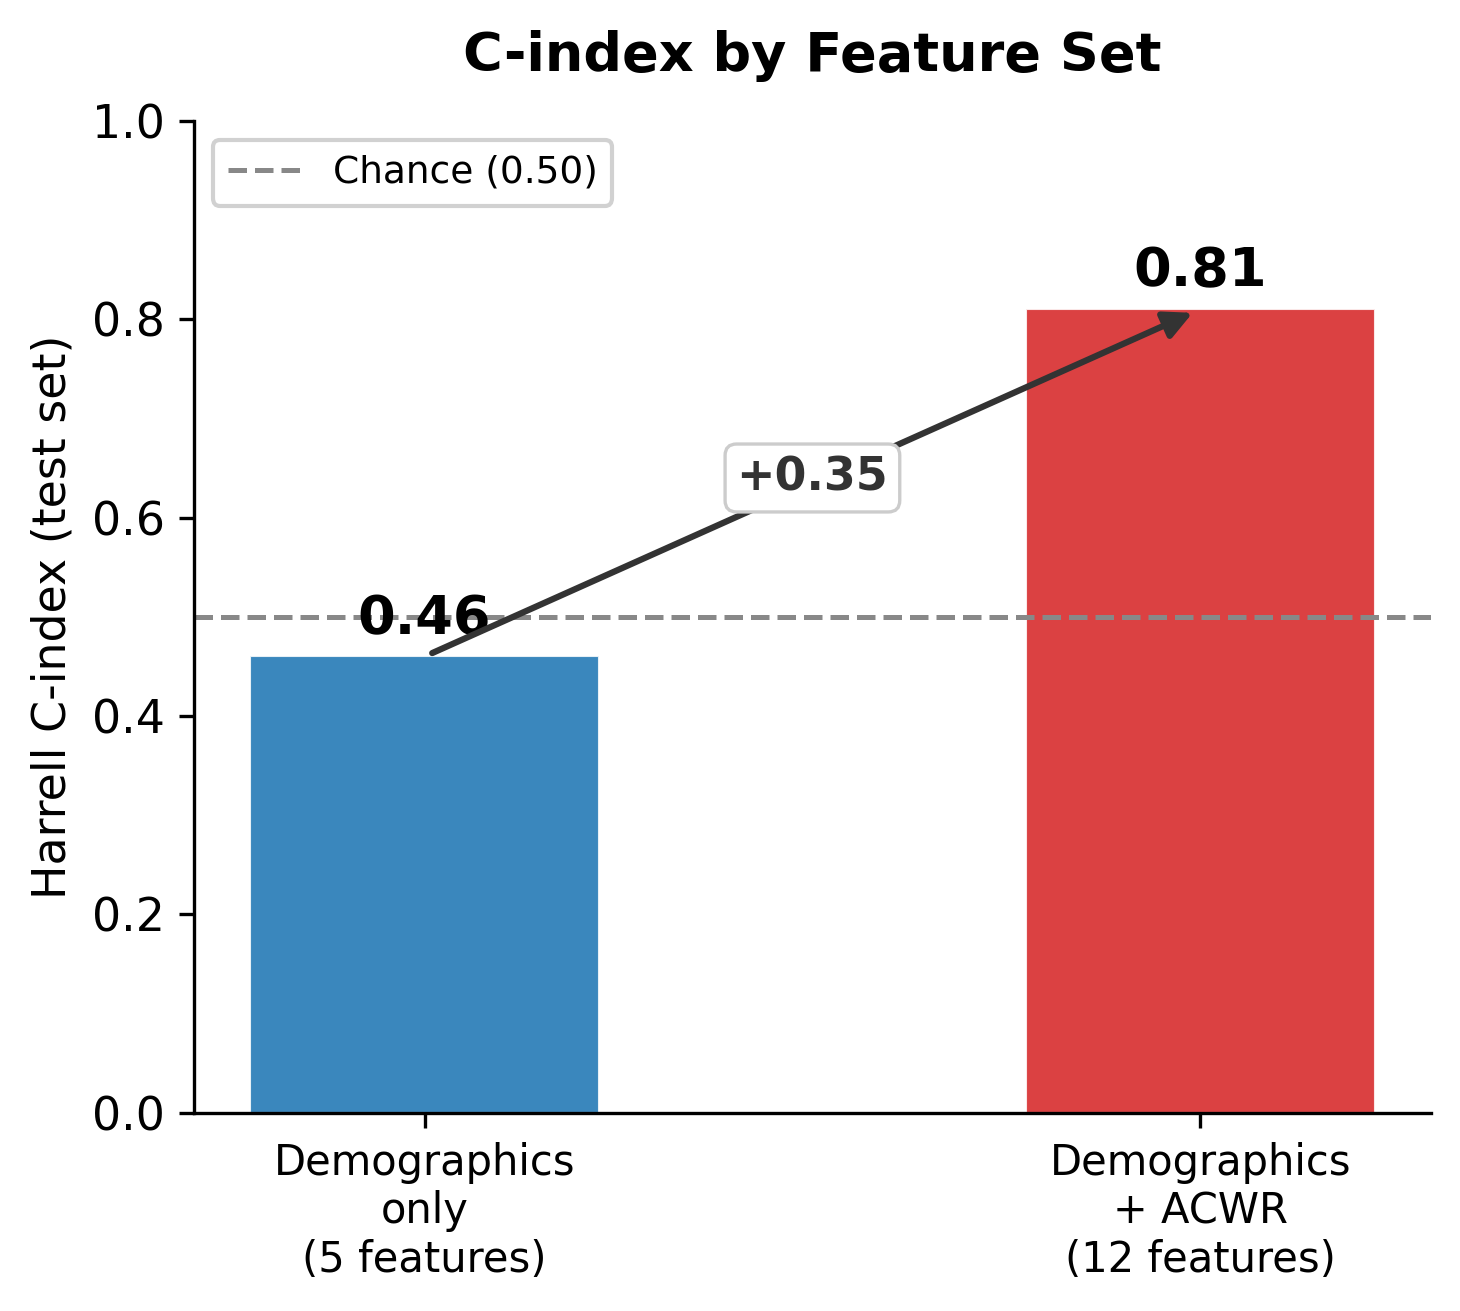
\includegraphics[width=0.75\linewidth]{cindex_comparison.png}
  \caption{\textbf{C-index by feature set.} Adding EWMA-ACWR workload features
  to a demographics-only baseline raises the held-out test C-index from 0.46
  to 0.81.  The dashed line marks chance-level discrimination (0.50).  The
  demographics-only model performs below chance, indicating that static
  anthropometric features systematically mis-rank matched patients.}
  \label{fig:cindex}
\end{figure}

\begin{figure}[h]
  \centering
  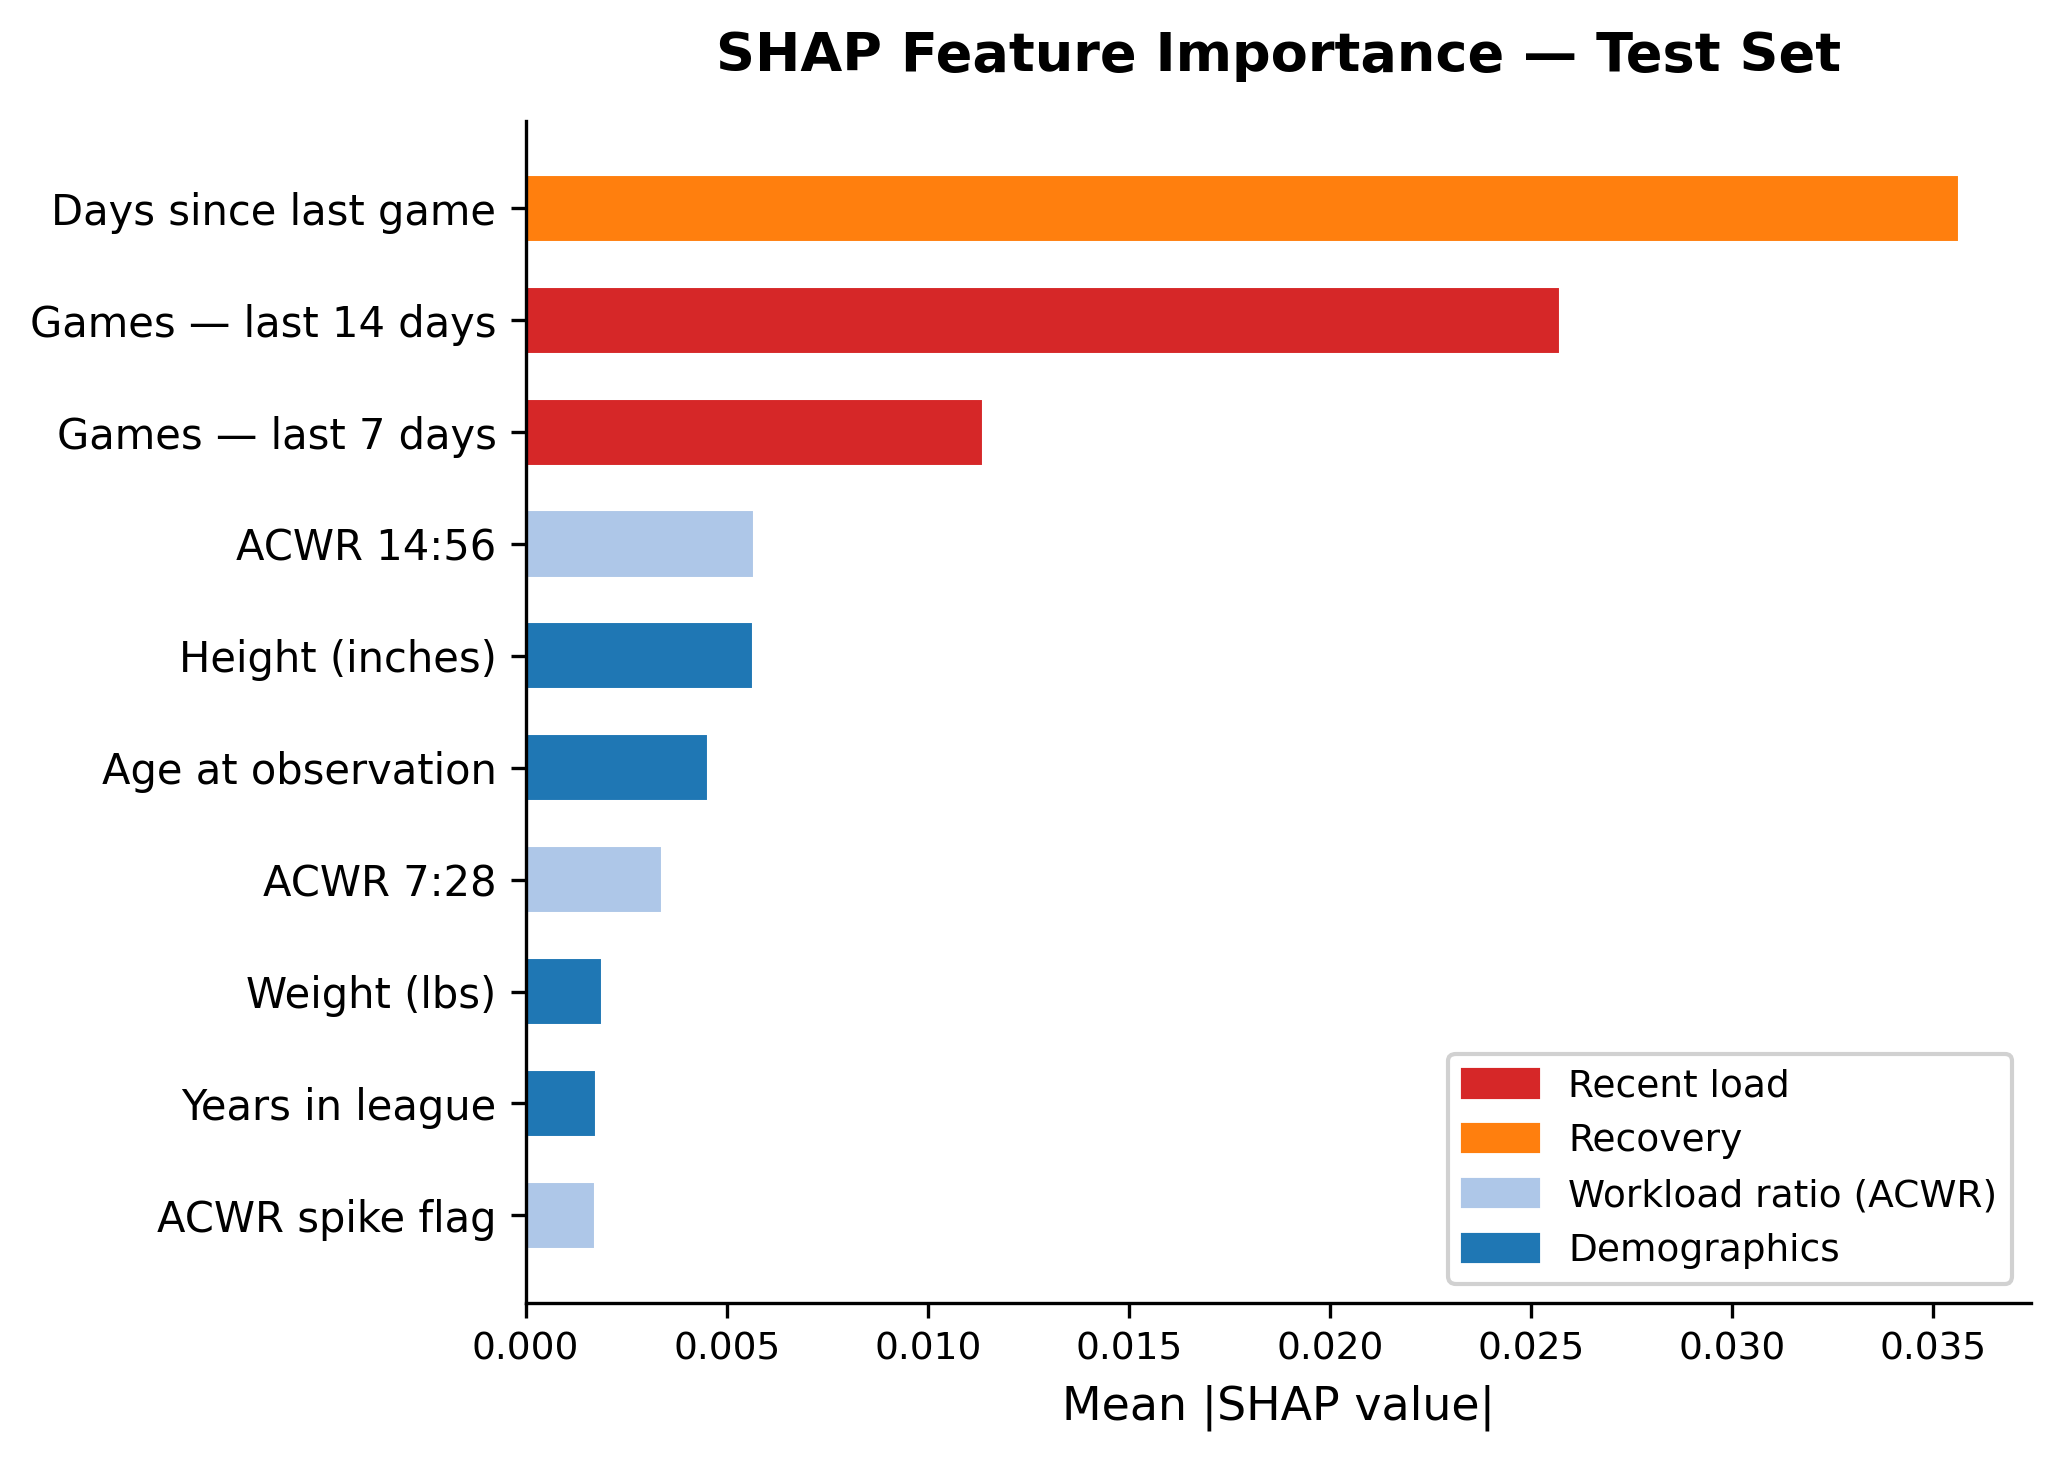
\includegraphics[width=0.80\linewidth]{shap_importance.png}
  \caption{\textbf{SHAP feature importance on the held-out test set.}  Features
  are coloured by category: recent load (red), recovery (orange), workload ratio
  (light blue), demographics (dark blue).  The top three features are
  all load/recovery metrics.  The first demographic feature (height) ranks 5th
  with mean $|\text{SHAP}|$ of 0.0052, approximately $6\times$ smaller than the
  top predictor (days since last game, 0.0298).}
  \label{fig:shap}
\end{figure}

\begin{figure}[h]
  \centering
  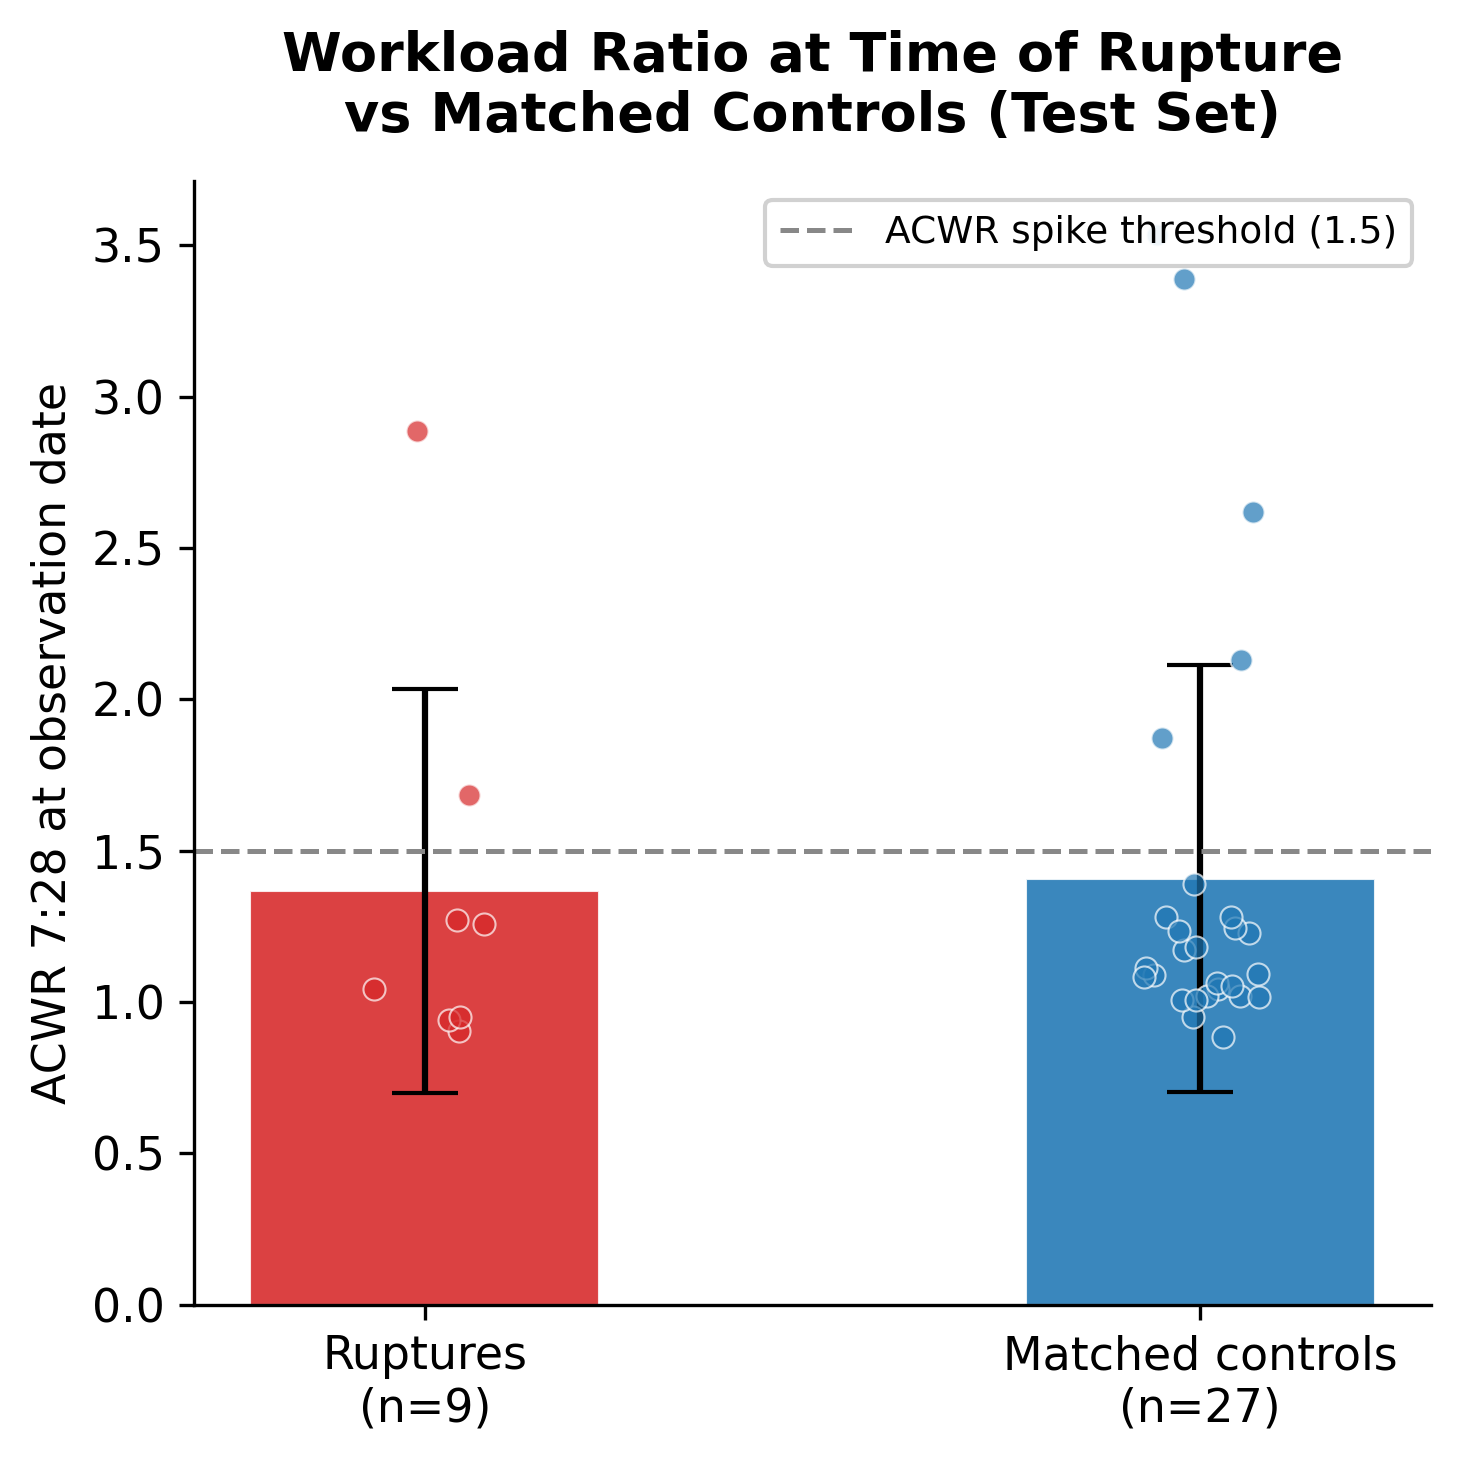
\includegraphics[width=0.60\linewidth]{acwr_vs_rupture.png}
  \caption{\textbf{ACWR 7:28 at observation date for rupture patients and
  matched controls (test set).}  Individual data points are shown with mean
  $\pm$ SD bars.  The dashed line marks the commonly used spike threshold
  ($\text{ACWR} > 1.5$).  Distributions overlap substantially (rupture
  $1.36 \pm 0.68$; control $1.41 \pm 0.65$), consistent with prior literature
  suggesting that temporal trajectory rather than point-in-time magnitude drives
  injury risk.  The survival model captures this dynamic through sequential
  game-log features, not through single-value ACWR thresholds.}
  \label{fig:acwr}
\end{figure}

\end{document}
